\documentclass[12pt,twoside]{article}   
\usepackage{../light}

\newcommand{\mfigure}[3]{\bigskip\centerline{\resizebox{#1}{#2}{\includegraphics{#3}}}\bigskip}

%\hidesolutions
\showsolutions

%\newcommand{\pr}[1]{\mathop{\textup{Pr}}\nolimits\left\(#1\right\)}
\newlength{\strutheight}
\newcommand{\prob}[1]{\mathop{\textup{Pr}} \nolimits \left( #1 \right)}
\newcommand{\prsub}[2]{\mathop{\textup{Pr}_{#1}}\nolimits\left(#2\right)}
\newcommand{\prcond}[2]{%
  \ifinner \settoheight{\strutheight}{$#1 #2$}
  \else    \settoheight{\strutheight}{$\displaystyle#1 #2$} \fi%
  \mathop{\textup{Pr}}\nolimits\left(
    #1\,\left|\protect\rule{0cm}{\strutheight}\right.\,#2
  \right)}
%\newcommand{\paren}[1]{\left(#1\right)}
\newcommand{\comment}[1]{}
\newcommand{\intersect}{\cap}
\newcommand{\union}{\cup}
\newcommand{\card}[1]{\lvert #1 \rvert}
%\newcommand{\pr}[1]{\Pr(#1)}
%\newcommand{\prob}[1]{\operatorname{Pr}(#1)}
%\newcommand{\prcond}[2]{\operatorname{Pr}(#1 \mid #2)}
%\newcommand{\prsub}[2]{\operatorname{Pr}_{#1}(#2)}
\newcommand{\cE}{\mathcal{E}}
\renewcommand{\setminus}{-}
\renewcommand{\complement}[1]{\overline{#1}}

\begin{document}

\problemset{11}{November 16, 2006}{\textit{Monday November 20 at 9 PM}}

%\insolutions{\stamp}

\begin{problem}[20 points]
We're interested in the probability that a randomly chosen poker hand (5
cards from a standard 52-card deck) contains cards from at most two suits.

%We use a few steps to attack the problem.

\bparts

\ppart What is an appropriate sample space to use for this problem?  What
are the outcomes in the event, $\cE$, we are interested in?  What are the
probabilities of the individual outcomes in this sample space?

\solution{The natural sample space to use consists of the $\binom{52}{5}$
possible poker hands.  The sample space is \emph{uniform}: Each hand is
equally likely and comes up with probability $1 / \binom{52}{5}$.}

\solution{
We define $\cE$ to be the subset of outcomes in which
the 5 cards on the outcome come from at most two suits.
}

\ppart  What is $\prob{\cE}$?

\solution{Since the sample space is uniform,
\[
\prob{\cE} = \frac{\card{\cE}}{\dbinom{52}{5}}.
\]
So we just need to determine the number of outcomes in $\cE$.  For this,
we resort to our usual counting techniques.  Doing it by cases works well.
There are three cases: 5 cards of one suit, 4 cards of one suit and 1 of
another suit, 3 cards of one suit and 2 of another suit.

For 5 of one suit, there are 4 ways to choose the suit and then
$\binom{13}{5}$ ways to choose 5 cards of that suit.

For 4 of one suit and 1 of another, there are 4 ways to choose the suit of
the 4 and $\binom{13}{4}$ ways to choose 4 cards of that suit, and there
are 3 remaining suits to choose for the 1, and 13 choices for the 1 card
of that suit.

Finally, for 3 of one suit and 2 of another, there are 4 ways to choose
the suit of the 3 and $\binom{13}{3}$ ways to choose 3 cards of that suit,
and there are 3 remaining suits to choose for the 2 cards, and
$\binom{13}{2}$ choices for the 2 cards of that suit.   So the total is
\[
4\cdot \binom{13}{5} + 4 \cdot \binom{13}{4} \cdot 3 \cdot 13 + 4 \cdot
\binom{13}{3} \cdot 3 \cdot \binom{13}{2},
\]
and the probability of at most two suits 
is
\[
\frac{4\cdot \dbinom{13}{5} + 4 \cdot \dbinom{13}{4} \cdot 3 \cdot 13 + 4 \cdot
\dbinom{13}{3} \cdot 3 \cdot \dbinom{13}{2}}{\dfrac{1}{\dbinom{52}{5}}}
 = 88/595 \approx 0.15.
\]

\iffalse
There are $\binom{4}{2}$ ways to choose two suits and $\binom{26}{5}$ ways
to choose five cards from these two suits.  But we need to be careful: some
of those $\binom{26}{5}$ choices might all come from the same suit.  These
hands will be triple-counted.  (For example, a hand containing \emph{only}
spades is counted once as a spades-hearts hand, a second time as a
spades-clubs hand, and a third time as a spades-diamonds hand.)  We can
correct for this triple-counting by subtracting off $2$ times the number of
hands that are triple-counted.  Since the number of hands with a single
suit is $4 \cdot \binom{13}{5}$, the number of hands with at most two suits
is
\[
\binom{4}{2} \cdot \binom{26}{5} - 2 \cdot 4 \cdot \binom{13}{5}.
\]
The probability that a random poker hand contains cards from at most
two suits is:
\begin{eqnarray*}
\prob{\cE}
        & = & \frac{\dbinom{4}{2} \cdot \dbinom{26}{5} -
                        2 \cdot 4 \cdot \dbinom{13}{5}}
                {\dbinom{52}{5}} \\
        & = & \frac{88}{595} \approx 0.15
\end{eqnarray*}
\fi

}

\eparts

\end{problem}

%%%%%%%%%%%%%%%%%%%%%%%%%%%%%%%%%%%%%%%%%%%%%%%%%%%%%%%%%%%%%%%%%%%%%%%%%%%%%%%%%%%%%%%%%%%



%\newpage

\begin{problem}


Suppose that {\em Let's Make a Deal} is played according to different
rules.  Now there are \underline{four} doors, with a prize hidden
behind one of them.  The contestant is allowed to pick a door.  The
host must then reveal a different door that has no prize behind it.
The contestant is allowed to stay with his or her original door or to
pick one of the other two that are still closed.  If the contestant
chooses the door concealing the prize in this second stage, then he or
she wins.

\bparts
\ppart 
Contestant Stu, a sanitation engineer from Trenton, New Jersey,
stays with his original door.  What is the probability that he wins
the prize?

The tree diagram is awkwardly large.  This often happens; in fact,
sometimes you'll encounter \textit{infinite} tree diagrams!  Try to
draw enough of the diagram so that you understand the structure of the
remainder.  If you still think you 
are drawing too much, consult with the course staff.

\solution{Let's make the same assumptions as in the original
problem:
%
\begin{enumerate}
\item The prize is equally likely to be behind each door.
\item The contestant is equally likely to pick each door initially,
regardless of the prize's location.
\item The host is equally likely to reveal each door that does not
conceal the prize and was not selected by the player.
\end{enumerate}
%
A partial tree diagram is shown below.  The remaining subtrees are
symmetric to the full-expanded subtree.
%
\begin{center}
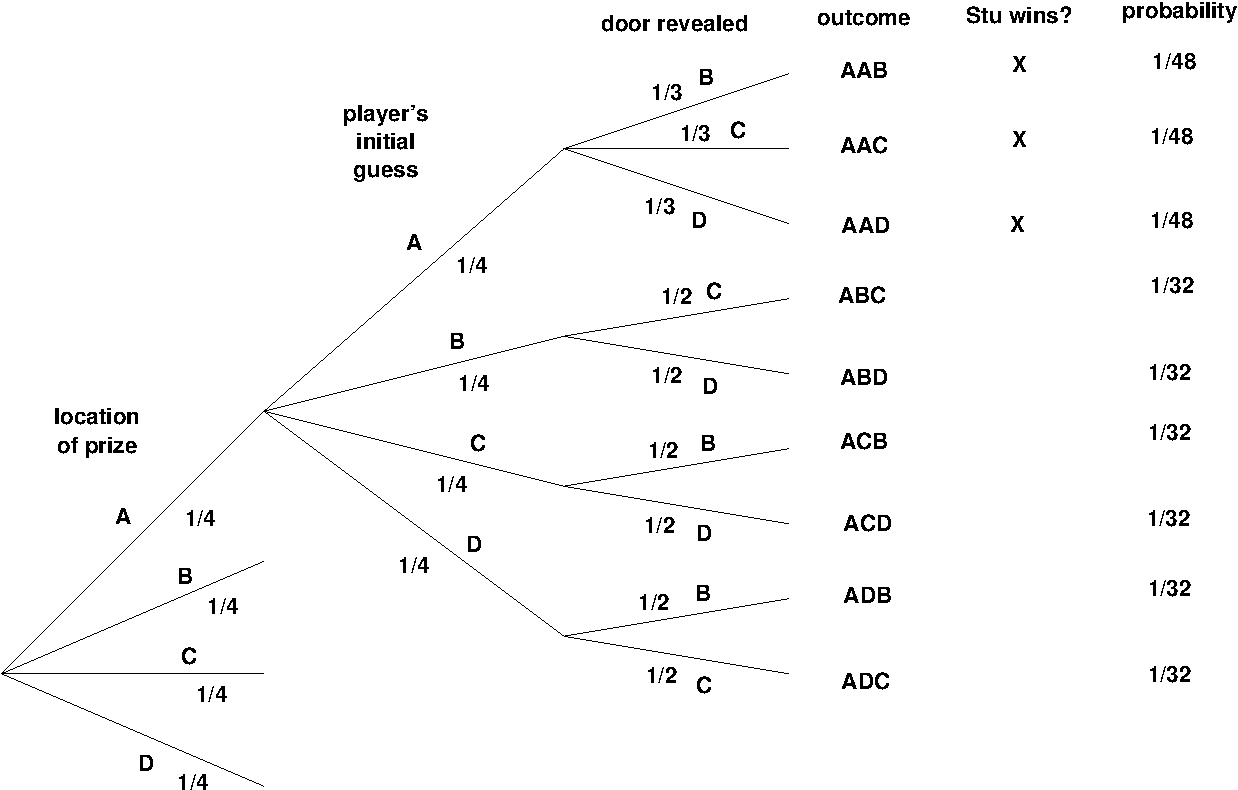
\includegraphics[width=6in]{four-door}
\end{center}
%
The probability that Stu wins the prize is:
%
\[
\pr{\text{Stu wins}} = 4 \cdot \left(\frac{1}{48} + \frac{1}{48} + \frac{1}{48}\right) = \frac{1}{4}
\]
%
We multiply by 4 to account for the four subtrees of which we've only
drawn one.}

\ppart 
Contestant Zelda, an alien abduction researcher from Helena,
Montana, switches to one of the remaining two doors with equal
probability.  What is the probability that she wins the prize?

\solution{A partial tree diagram is worked out below.
%
\begin{center}
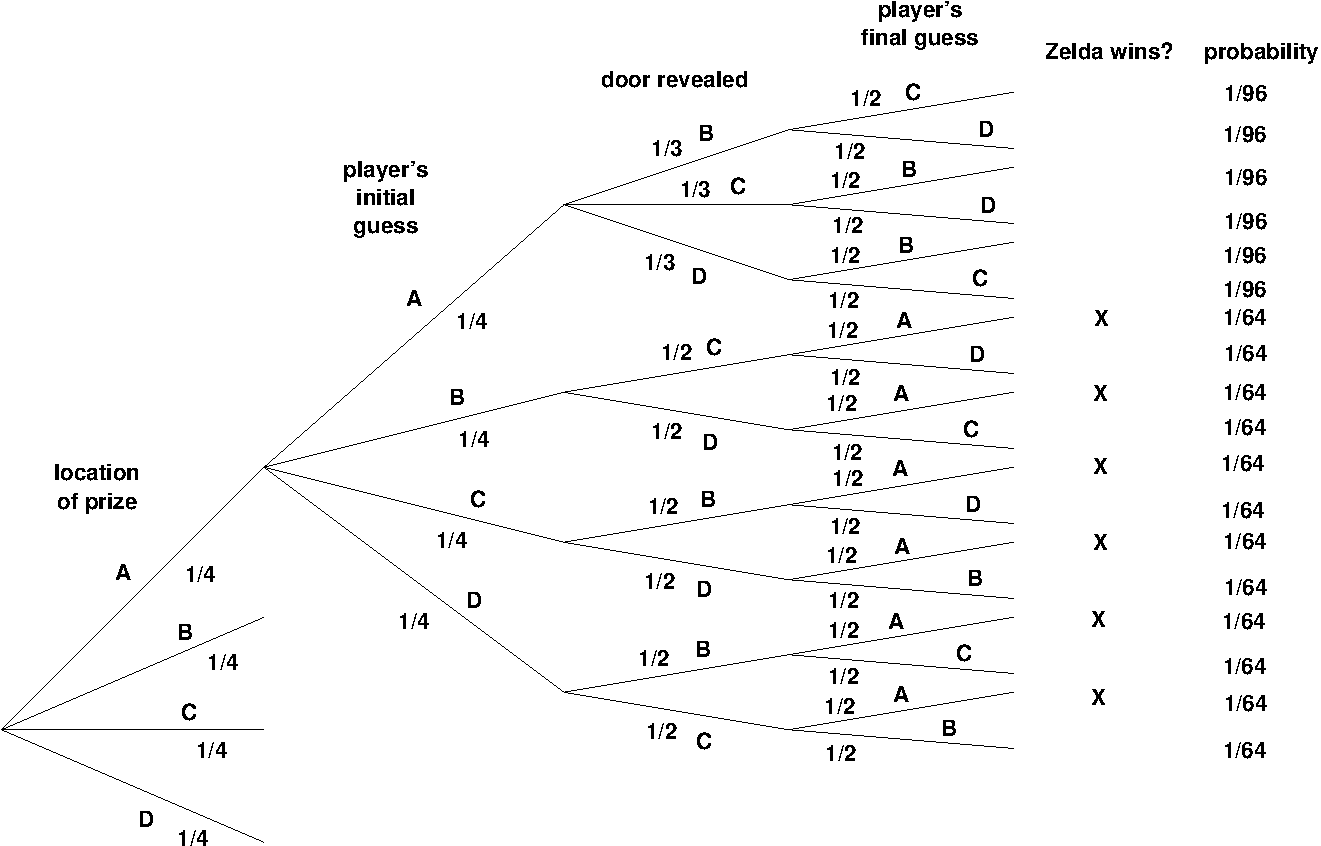
\includegraphics[width=6in]{four-doorb}
\end{center}
%
The probability that Zelda wins the prize is:
%
\[
\pr{\text{Zelda wins}} = 4 \cdot \left( \frac{1}{64} + \frac{1}{64} + \frac{1}{64} + \frac{1}{64} + \frac{1}{64} + \frac{1}{64} \right) = \frac{3}{8}
\]
}


\ppart
Let's consider another variation of the four-doors problem.  Suppose
that Carol always opens the \textit{lowest-numbered} door possible
with the restriction that she can neither reveal the prize nor open
the door that the player picked.

This gives contestant Mergatroid--- an engineering student from
Cambridge, MA--- just a little more information about the location of
the prize.  Suppose that Mergatroid always switches to the
lowest-numbered door, excluding his initial pick and the one Carol
opened.  What is the probability that he wins the prize?

(Interestingly, in the three-door problem, the contestant gains
\textit{no} advantage if Carol always opens the lowest-numbered door
available.)  

\solution{
A tree diagram is worked out below.
%
\begin{center}
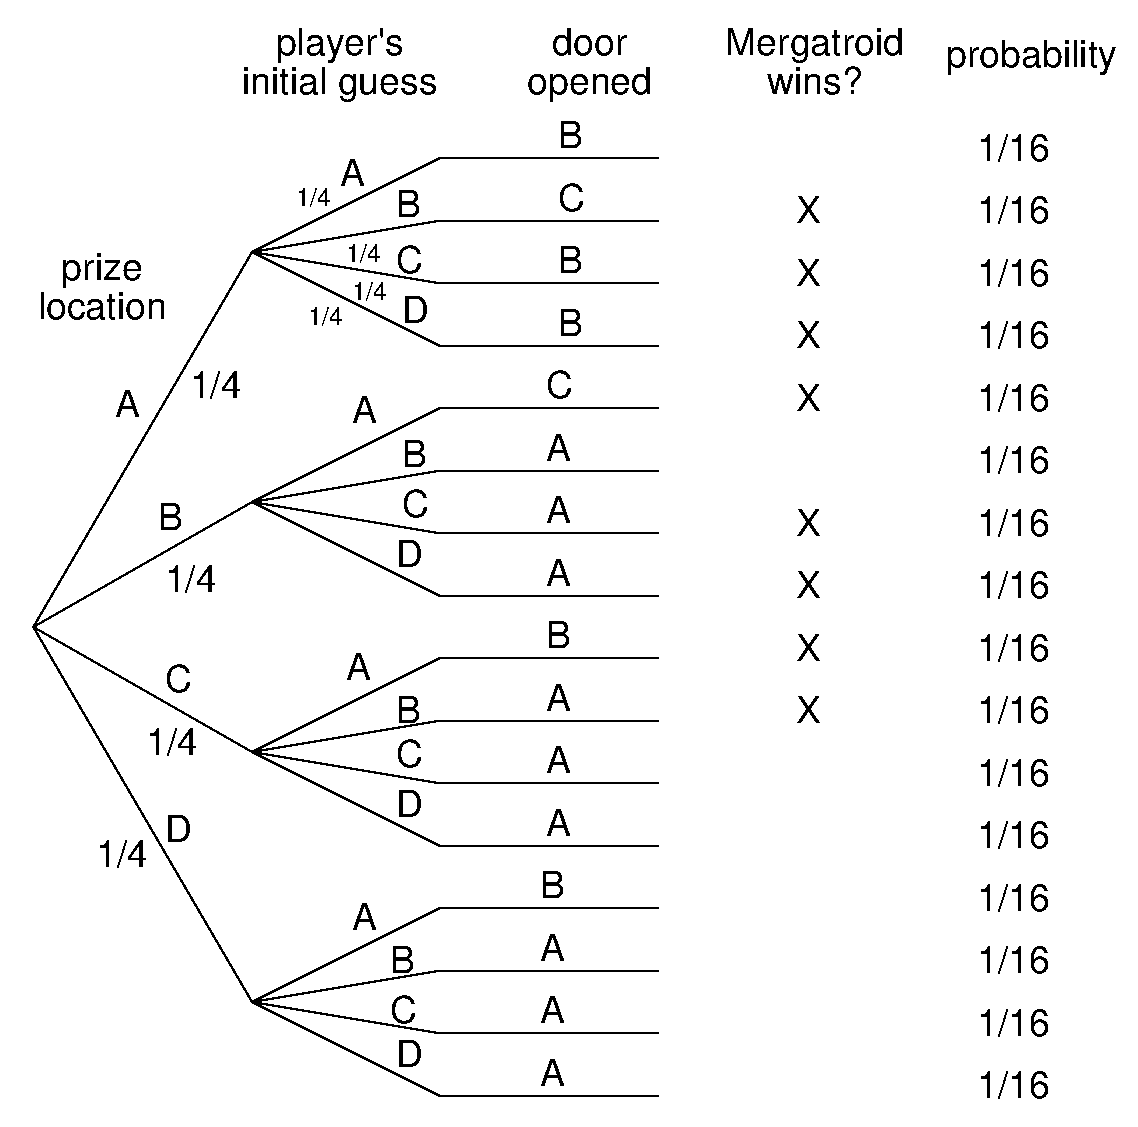
\includegraphics[height=3.5in]{carol}
\end{center}
%
The probability that Mergatroid wins is:
%
\[
\pr{\text{win}} = 8 \cdot \frac{1}{16} = \frac{1}{2}
\]
}


\eparts

\end{problem}


%%%%%%%%%%%%%%%%%%%%%%%%%%%%%%%%%%%%%%%%%%%%%%%%%%%%%%%%%%%%%%%%%%%%%%%%%%%%%%%

%%%%%%%%%%%%%%%%%%%%%%%%%%%%%%%%%%%%%%%%%%%%%%%%%%%%%%%%%%%%%%%%%%%%%%%%%%%
%\newpage

\begin{problem}[20 points]
Recall the strange dice from lecture:
\begin{center}
%\mfigure{!}{3.5in}{lec2-dice}
\mfigure{!}{2in}{../figures/dice}
\end{center}
In lecture we proved that if we roll each die once, then die $A$ beats $B$ more often, die $B$ beats die $C$ more often, and die $C$ beats die $A$ more often. Thus, contrary to our intuition, the ``beats'' relation $>$ is not transitive. That is, we have $A > B > C > A$.

We then looked at what happens if we roll each die twice, and add the result. In lecture, we showed that rolling die $B$ twice is more likely to win, i.e., have a larger sum, than rolling die $A$ twice, which is the opposite of what happened if we were to just roll each die once! In fact, we will show that the ``beats'' relation reverses in this game, that is, $A < B < C < A$, which is very counterintuitive!

\iffalse
\bparts

\ppart 
\fi

Show that rolling die $C$ twice is more likely to win than rolling die $B$ twice.

\solution{We draw the sample space. In the figure, it should be understood that the tree corresponding to $B$ is connected to each leaf of the tree corresponding to $C$. 
\begin{center}
\mfigure{!}{3in}{dieSum2}
\end{center}
As in lecture, there are $81$ leaves and the space is uniform, i.e., each outcome occurs with probability $(1/3)^4 = 1/81$. Let's work out the chances of winning. The sum of the two rolls of the $B$ die is equally likely to be any element of the following multiset:
$$S_B = \{2, 6, 6, 10, 10, 10, 14, 14, 18\}.$$
The sum of the two rolls of the $C$ die is equally likely to be any element of the following multiset:
$$S_C = \{6, 7, 7, 8, 11, 11, 12, 12, 16\}.$$
We can treat each outcome as a pair $(x,y) \in S_B \times S_C$, where $C$ wins iff $y > x$. If $y = 6$, there is $1$ value of $x$, namely $x = 2$, for which $y > x$. Continuing the count in this way, the number of pairs for which $y > x$ is $$1 + 3 + 3 + 3 + 6 + 6 + 6 + 6 + 8 = 42,$$
while there are $2$ ties and $37$ cases where $B$ wins. Thus, rolling die $C$ twice is more likely to win than rolling die $B$ twice.
}

\iffalse
\ppart Show that rolling die $A$ twice is more likely to win that rolling die $C$ twice.

\solution{We draw the sample space. In the figure, it should be understood that the tree corresponding to $C$ is connected to each leaf of the tree corresponding to $A$. 
\begin{center}
\mfigure{!}{3in}{dieSum3}
\end{center}
As in lecture, there are $81$ leaves and the space is uniform, i.e., each outcome occurs with probability $(1/3)^4 = 1/81$. Let's work out the chances of winning. The sum of the two rolls of the $C$ die is equally likely to be any element of the following multiset:
$$S_C = \{6, 7, 7, 8, 11, 11, 12, 12, 16\}.$$
The sum of the two rolls of the $A$ die is equally likely to be any element of the following multiset:
$$S_A = \{4, 8, 8, 9, 9, 12, 13, 13, 14\}.$$
We can treat each outcome as a pair $(x,y) \in S_C \times S_A$, where $A$ wins iff $y > x$. If $y = 4$, there is no $x$ for which $y > x$. If $y = 8$, there are $3$ values of $x$, namely $x = 6, 7, 7$, for which $y > x$. Continuing the count in this way, the number of pairs for which $y > x$ is $$0 + 3 + 3 + 4 + 4 + 6 + 8 + 8 + 8 = 44,$$
while a similar count shows that there are only $33$ pairs for which $x > y$, and there are $4$ ties. Thus, rolling die $A$ twice is more likely to win than rolling die $C$ twice.
}

\eparts 
\fi
\end{problem}
%\newpage

\begin{problem}[20 points] \label{Identities}
Prove the following probabilistic identity, referred to as the {\bf Union
Bound}.  You may assume the theorem
that the probability of a union of \emph{disjoint} sets is the sum of their
probabilities.

\iffalse
\bparts

\ppart \label{setminus}
$\prob{A \setminus B} = \prob{A} - \prob{A \intersect B}$.

\solution{
Any set, $A$, is the disjoint union of $A \setminus B$ and $A \intersect
B$, for any set, $B$.
Thus, 
\[
\prob{ A }= 
\prob{A \setminus B} + \prob{A \intersect B}.
\]
Subtracting $\prob{A \intersect B}$ from both sides gives the desired result.
}


\ppart \label{inclexcl}
The \emph{Inclusion-Exclusion Rule for probability}:
\begin{equation}\label{inclexcleq}
\prob{A \union B} = \prob{A} + \prob{B} - \prob{A \intersect B}.
\end{equation}


\solution{ The proof exactly mirrors the proof of the original
inclusion-exclusion rule given in earlier Notes.  Namely, for any sets
$A,B$, the set $A \union B$ is the disjoint union of $A-B$ and $B$, so
\begin{align*}
\prob{A \union B}
 &= \prob{A \setminus B} + \prob{B} & \text{(disjoint union)}\\
 &= (\prob{A} - \prob{A \intersect B}) + \prob{B} & \text{(by~\eqref{setminus})}\\
 &= \prob{A} + \prob{B} - \prob{B \intersect A}.
\end{align*}
}


\ppart  
The \term{Union Bound:}
\fi

Let $A_1, \dots, A_n$ be a collection of events.  Then
\[
\prob{A_1 \union A_2 \union \cdots \union A_n} \leq \sum_{i=1}^n
\prob{A_i}.
\]
\emph{Hint:} Induction.

\solution{
For all $n \geq 1$, let $P(n)$ be the proposition that the claim is true.

\textit{Base case:} Trivially $\prob{A_1} \leq \prob{A_1}$, so $P(1)$ is true.

\textit{Induction step:} Assume that $P(n)$ is true and show $P(n+1)$ for
$n \geq 1$.
\begin{align*}
\prob{ A_1 \union A_2 \union \cdots \union A_{n+1}} 
 &= \prob{(A_1 \union A_2 \union \cdots \union A_{n}) \union A_{n+1}} \\
 &= \prob{A_1 \union A_2 \union \cdots \union A_{n}} + \prob{A_{n+1}} \\
 &\quad - \prob{(A_1 \union A_2 \union \cdots \union A_{n}) \intersect A_{n+1}}
 &\text{(by~Inclusion-Exclusion)}\\
 &\leq \prob{A_1 \union A_2 \union \cdots \union A_{n}} + \prob{A_{n+1}}\\
 &\leq \sum_{i=1}^{n} \prob{A_{i}} + \prob{A_{n+1}} &\text{(by Ind. Hyp.)} \\
 &= \sum_{i=1}^{n+1} \prob{A_{i}} 
\end{align*}
Thus $P(n)$ is true and the result follows by induction.
}

\iffalse
\eparts
\fi

\end{problem}

%%%%%%%%%%%%%%%%%%%%%%%%%%%%%%%%%%%%%%%%%%%%%%%%%%%%%%%%%%%%%%%%%%%%%%%%%%%%%%%%%%%%%%%%%%%%%%
\iffalse
\begin{problem}[20 points] \label{relative}

Most probability identities continue to hold when all probabilities are
conditioned on the same positive probability event, $C$.  For example, the
Inclusion-Exclusion rule~\eqref{inclexcleq} can be conditioned on $C$ to
become the Conditional Inclusion-Exclusion Rule:
\begin{equation}\label{cie}
\prcond{A \union B}{C} = \prcond{A}{C} + \prcond{B}{C} - \prcond{A \intersect B}{C}.
\end{equation}

\bparts

\ppart Define a new function, $\prsub{C}{}$ by the
rule that
\begin{definition*}%\label{defprs}
\[
\prsub{C}{A} = \prcond{A}{C}.
\]
\end{definition*}
Prove that for any positive probability event, $C$, the function
$\prsub{C}{}$ is another probability measure (on the same sample space).

\iffalse \textit{Hint:} Review the definition of a probability space in the
lecture notes.
\hyperref{http://theory.lcs.mit.edu/classes/6.042/spring02/handouts/lectures/ln9.pdf}
{ln9}{probsp}{Notes 9, Definition 5.2}.
\fi


\solution{
The sample space, $S$, for the new probability space has not
changed.  Note that $\prsub{C}{}$ is defined on events, so we define the
probability of an outcome, $s \in S$, to be the probability of the event
$\set{s}$.

We must must show for the new probability function, $\prsub{C}{}$,
that
\begin{enumerate}

\item the probability of each outcome is nonnegative,

\item\label{S} the sum of the probabilities of all the outcomes in $S$ is 1, and

\item\label{A} the probability of an event is the sum of the probabilities
of its outcomes.

\end{enumerate}
\begin{proof}

To show that outcome probabilities are nonegative, we note that
for any outcome $s \in S$, we have
\[
\prsub{C}{s}= \prsub{C}{\set{s}} = \prcond{\set{s}}{C} = \frac{\pr{\set{s} \cap
C}}{\pr{C}},
\]
and the last quantity is nonnegative because it is a quotient of
nonnegative quantities.


Next we observe that
\[
\prsub{C}{S} = 1
\]
because

\begin{align*}
\prsub{C}{S} & = \prcond{S}{C}
                     & \text{(Def of $\prsub{C}{}$)}\\
             & = \frac{\pr{S \cap C}}{\pr{C}}
                     & \text{(Def of $\prcond{}{C}$)}\\
             & = \frac{\pr{C}}{\pr{C}} = 1
                     & (C \subseteq S).
\end{align*}


So if the probability of $S$ is the sum of the probability of the
outcomes, it follows that the sum of the outcome probabilities is 1, that
is,~\ref{S}.\ holds.

So it remains only to prove~\ref{A}., namely, that for any event, $A$,
\[
\prsub{C}{A} = \sum_{s \in A} \prsub{C}{s}.
\]

This follows because
\begin{align*}
\prsub{C}{A} & = \prcond{A}{C}
                     & \text{(Def of $\prsub{C}{}$)}\\
             & = \frac{\pr{A \cap C}}{\pr{C}}
                     & \text{(Def of $\prcond{}{C}$)}\\
             & = \frac{\sum_{s \in (A \cap C)} \pr{s}}{\pr{C}}
                       &\text{($\pr{E} = \sum_{s \in E} \pr{s}$ for any $E$)}\\
             & = \sum_{s \in (A \cap C)} \frac{\pr{s}}{\pr{C}}\\
             & = \sum_{s \in A} \frac{\pr{\set{s} \cap C}}{\pr{C}}
                & \text{($\set{s} \cap C = \emptyset$ unless $s \in C$)}\\
             & = \sum_{s \in A} \prcond{\set{s}}{C}
                     & \text{(Def of $\prcond{}{C}$)}\\
             & = \sum_{s \in A} \prsub{C}{s}
                     & \text{(Def of $\prsub{C}{}$)}.
\end{align*}

\end{proof}
}


\ppart Use part~(a) to give a simple proof of the Sum Rule conditioned on
$C$.  Namely, suppose $A$ is the disjoint union of sets
$A_1,A_2,\dots,A_n$.  Prove that
\begin{equation*}
\prcond{A}{C} = \sum_{i}^n {\prcond{A_i}{C}}.
\end{equation*}

\solution{
\begin{align*}
\prcond{A}{C} & = \prcond{\bigcup_{i}^n A_i}{C}\\
    &= \prsub{C}{\bigcup_i^n A_i}
            & \text{Def of $\prsub{C}{}$}\\
    &= \sum_i^n \prsub{C}{A_i} & \text{(Sum Rule for $\prsub{C}{}$)}\\
    &=  \sum_{i}^n {\prcond{A_i}{C}} &
           \text{Def of $\prsub{C}{}$}.
\end{align*}

}

\eparts

\end{problem}
\fi



\begin{problem} \textit{Finalphobia} is a rare
disease in which the victim has the delusion that he or she is being
subjected to an intense mathematical examination.
%
\begin{itemize}
\item A person selected uniformly at random has finalphobia with probability
$1/100$.
\item A person with finalphobia has shaky hands with probability $9/10$.
\item A person without finalphobia has shaky hands with probability $1/20$.
\end{itemize}
%
What is the probablility that a person selected uniformly at random
has finalphobia, given that he or she has shaky hands?

\solution{
Let $F$ be the event that the randomly-selected person has
finalphobia, and let $S$ be the event that he or she has shaky hands.
A tree diagram is worked out below:
%
\begin{center}
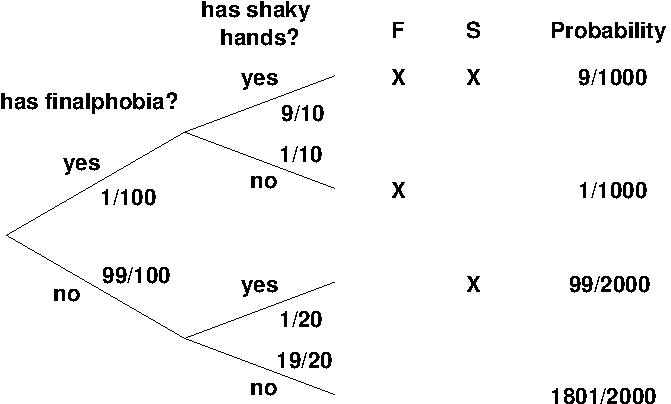
\includegraphics{finalphobia}
\end{center}
%
The probability that a person has finalphobia, given that he or she
has shaky hands is:
%
\begin{align*}
\prcond{F}{S}
    & = \frac{\pr{F \cap S}}{\pr{S}} \\
        & = \frac{9/1000}{9/1000 + 99/2000} \\
	    & = \frac{18}{18+99} \\
	        & = \frac{18}{117}
		\end{align*}

		So, while it's true that someone with shaky hands is five times more
		likely to have finalphobia than someone with steady hands, it remains a
		poor bet --about 1 in 5 --that someone with shaky hands actually has does
		have finalphobia.}

		\end{problem}


%\begin{problem}
%Outside of their hum-drum duties as 6.042 TAs, Arvind is trying to
%learn to levitate using only intense concentration and Amy is
%launching a ``Wibowo 2008'' presidential campaign.  Suppose that Arvind's
%probability of levitating is $1/6$, Amy's chance of becoming
%president is $1/4$, and the success of one does not alter the other's
%chances.
%
%\bparts
%
%\ppart If at least one of them succeeds, what is the probability that
%Arvind learns to levitate?
%
%\solution{Let $L$ be the event that Arvind learns to levitate, and let
%$P$ be the event that Amy becomes president.  We can work out the
%desired probability as follows:
%%
%\begin{align*}
%\prcond{L}{(L \cup P)}
%	& = \frac{\pr{L \cap (L \cup P)}}{\pr{L \cup P}} \\
%	& = \frac{\pr{L}}{1 - \pr{\overline{L} \cap \overline{P}}} \\
%	& = \frac{1/6}{1 - (1 - 1/6)(1 - 1/4)} \\
%	& = \frac{4}{9}
%\end{align*}
%%
%The first step uses the definition of conditional probability.  In the
%second step, we rewrite both the top and bottom of the fraction using
%set identities.  Then we substitute in the given probability and
%simplify.}
%
%\ppart If at most one of them succeeds, what is the probability that
%Amy becomes the president of the United States?
%
%\solution{
%Define events $L$ and $P$ as before.
%%
%\begin{align*}
%\prcond{P}{\paren{\overline{L} \cup \overline{P}}}
%	& = \frac{\pr{P \cap \paren{\overline{L} \cup \overline{P}}}}
%		{\pr{\overline{L} \cup \overline{P}}} \\
%	& = \frac{\pr{P \cap \overline{L}}}
%		{1 - \pr{L \cap P}} \\
%	& = \frac{(1/4) \cdot (5/6)}{1 - (1/6) \cdot (1/4)} \\
%	& = \frac{5}{23}
%\end{align*}
%}
%
%\ppart If exactly one of them succeeds, what is the probability that
%it is Arvind?
%
%\solution{
%\begin{align*}
%\prcond{L}{\paren{\paren{L \cap \overline{P}} \cup \paren{\overline{L} \cap P}}}
%	& = \frac{\pr{L \cap \overline{P}}}
%		{\pr{(L \cap \overline{P}) \cup
%		(\overline{L} \cap P)}} \\
%	& = \frac{(1/6) \cdot (3/4)}
%		{(1/6) \cdot (3/4) + (5/6) \cdot (1/4)} \\
%	& = \frac{3}{8}
%\end{align*}
%}
%
%\eparts
%\end{problem}
%
\end{document}
